\section{Visualization of TensorFlow Graphs}\label{sec:visual}

High level discussion of what visualization is and why it is important

\subsection{TensorBoard Features}\label{sec:visual-features}

Interesting are features:

1.
2.
3.
4.
5.

\subsection{TensorBoard in Practice}\label{sec:visual-code}

To integrate, three elements are

1. name_scope context manager
2. scalar_summary
3. histogram_summary
4. SummaryWriter

Example

\begin{figure}[h!]
  \centering
  \begin{subfigure}[h]{0.5\textwidth}
    \centering
    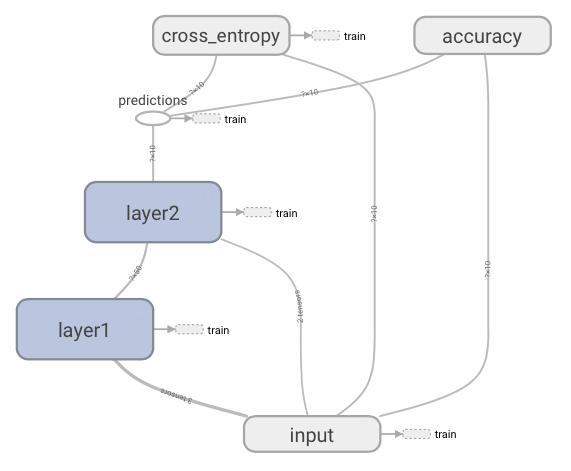
\includegraphics[scale=0.4]{no-train}
   \caption{}
   \label{fig:tensorboard-a}
  \end{subfigure}

  \vspace{0.3cm}

  \begin{subfigure}[h]{0.5\textwidth}
    \centering
    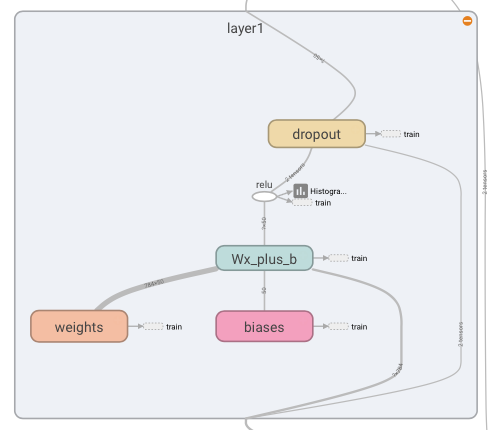
\includegraphics[scale=0.4]{layer1}
    \caption{}
    \label{fig:tensorboard-b}
  \end{subfigure}

  \vspace{0.3cm}

  \begin{subfigure}[h]{0.2\textwidth}
    \centering
    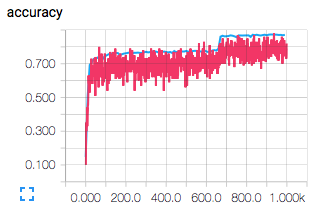
\includegraphics[scale=0.35]{accuracy}
    \caption{}
    \label{fig:tensorboard-c}
  \end{subfigure}
  %
  \begin{subfigure}[h]{0.2\textwidth}
    \centering
    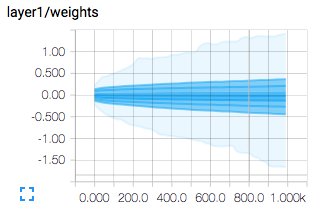
\includegraphics[scale=0.35]{blue-weights}
    \caption{}
    \label{fig:tensorboard-d}
  \end{subfigure}
  \caption{Foo}
  \label{fig:tensorboard}
\end{figure}

%%% Local Variables:
%%% mode: latex
%%% TeX-master: "../paper"
%%% End: